% Created 2017-11-25 Sat 17:12
% Intended LaTeX compiler: pdflatex
\documentclass[presentation]{beamer}
\usepackage[utf8]{inputenc}
\usepackage[T1]{fontenc}
\usepackage{graphicx}
\usepackage{grffile}
\usepackage{longtable}
\usepackage{wrapfig}
\usepackage{rotating}
\usepackage[normalem]{ulem}
\usepackage{amsmath}
\usepackage{textcomp}
\usepackage{amssymb}
\usepackage{capt-of}
\usepackage{hyperref}
\usepackage{minted}
\setminted[ipython]{frame=lines, fontsize=\tiny}
\setminted[python]{frame=lines, fontsize=\tiny}
\setminted[haskell]{frame=lines, fontsize=\tiny}
\usefonttheme[onlymath]{serif}
\usetheme{Boadilla}
\date{}
\title{GP - Rasmussen \& Williams - Ch. 2: Regression}
\hypersetup{
 pdfauthor={},
 pdftitle={GP - Rasmussen \& Williams - Ch. 2: Regression},
 pdfkeywords={},
 pdfsubject={},
 pdfcreator={Emacs 24.5.1 (Org mode 9.1.1)}, 
 pdflang={English}}
\begin{document}

\maketitle
\begin{frame}{Outline}
\tableofcontents
\end{frame}



\section{Regression}
\label{sec:orgfdbac7e}
\subsection{Sampling from prior}
\label{sec:org8ef209e}
\begin{frame}[label={sec:org86e9e82}]{GP prior}
\begin{eqnarray} \label{eg:GP}
k({x},{y}) & = & \mathrm{exp}( -\tfrac{1}{2}|{x}-{y}|^2) \\
\mathbf{f} & \sim & \mathcal{N}(\mathbf{0}, K(\mathbf{x}, \mathbf{x}))
\end{eqnarray}
\end{frame}


\begin{frame}[fragile,label={sec:orgabe92c4}]{Sampling from prior: Python code}
 \begin{minted}[]{ipython}
from numpy import sum, eye, exp #, zeros
from numpy.linalg import cholesky
from numpy.random import normal #, multivariate_normal

def rbf(length_scale):
    def k(x,y):
        if len(x.shape)==1:
            d = 1
        else:
            d  = x.shape[1]
        lx = x.shape[0]
        ly = y.shape[0]
        dists =  sum(((x.T.reshape([d,lx,1]) -  y.T.reshape([d,1,ly]))/length_scale)**2,0)
        return exp(-.5 * dists)
    return k

def genSamplesSimple(x, k):
    n = x.shape[0]
    L = cholesky(k(x,x)+eye(n)*1e-8)
    return L.dot(normal(size=n))
# Same as:
#    return multivariate_normal(zeros(n), k(x,x) + eye(n)*1e-8)
\end{minted}

\begin{minted}[]{python}
from matplotlib.pyplot import figure, plot, savefig, close, legend
from numpy import linspace

figure()
x = linspace(-5,5,150)
k = rbf(1)
for i in range(3): plot(x, genSamplesSimple(x,k));
\end{minted}
\end{frame}



\begin{frame}[label={sec:org509ea7a}]{Random functions in 1D}
\begin{center}
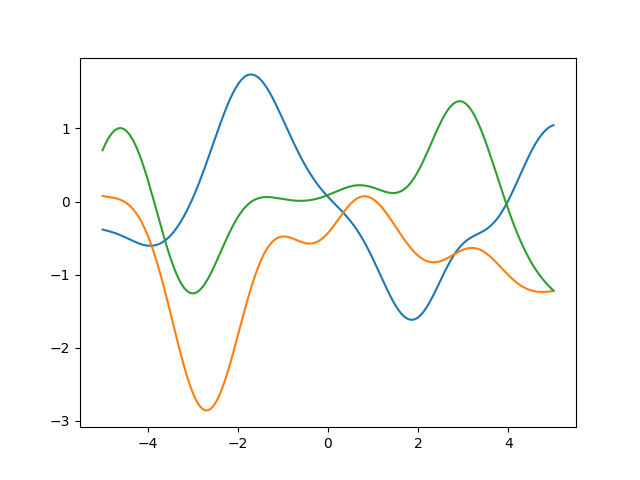
\includegraphics[width=.9\linewidth]{images/fig01.png}
\end{center}
\end{frame}


\begin{frame}[fragile,label={sec:org47395f3}]{Different length scales}
 \begin{columns}
\begin{column}{0.45\columnwidth}
\begin{minted}[]{python}
scales = [0.2, 1, 5]
for i in scales:
  plot(x, genSamplesSimple(x,rbf(i)))
legend(scales)
\end{minted}
\end{column}


\begin{column}{0.45\columnwidth}
\begin{center}
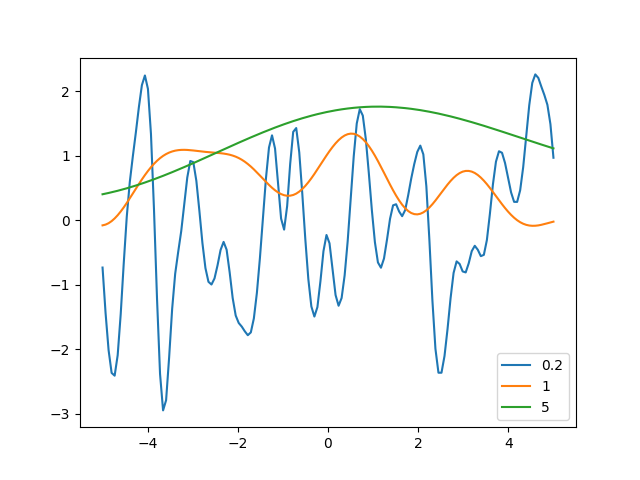
\includegraphics[width=.9\linewidth]{images/fig02.png}
\end{center}
\end{column}
\end{columns}
\end{frame}

\begin{frame}[fragile,label={sec:org1e870dc}]{Two dimensions}
 \begin{columns}
\begin{column}{0.4\columnwidth}
\begin{minted}[]{python}
from numpy import meshgrid, concatenate

x = linspace(5, -5, 50)
xx, yy = meshgrid(x, x)
xy = concatenate([xx.reshape([1, -1]),
                  yy.reshape([1, -1])]).T
z = genSamplesSimple(xy, rbf(2)).reshape([50, 50])
\end{minted}


\begin{minted}[]{python}
fig = figure()
ax = fig.gca(projection='3d')
ax.plot_surface(xx, yy, z, rstride=8,
                cstride=8, alpha=0.3)
cset = ax.contour(xx, yy, z, zdir='z',
                  offset=-2.5, cmap=cm.coolwarm)
cset = ax.contour(xx, yy, z, zdir='x',
                  offset=-5, cmap=cm.coolwarm)
cset = ax.contour(xx, yy, z, zdir='y',
                  offset=5, cmap=cm.coolwarm)

ax.set_xlabel('X')
ax.set_xlim(-5, 5)
ax.set_ylabel('Y')
ax.set_ylim(-5, 5)
ax.set_zlabel('Z')
ax.set_zlim(-2.5, 2.5)
\end{minted}
\end{column}



\begin{column}{0.6\columnwidth}
\begin{center}
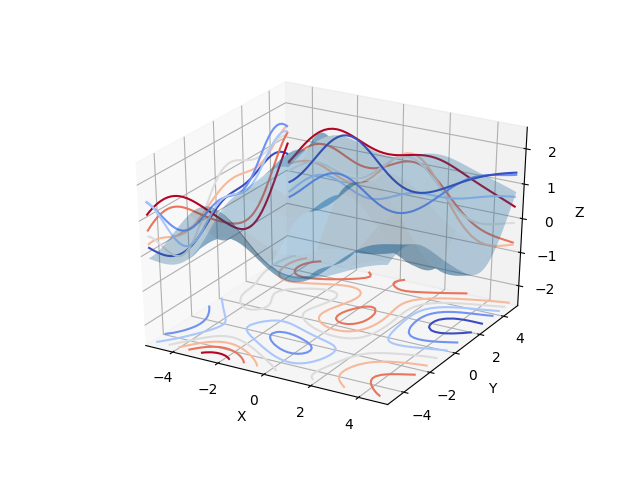
\includegraphics[width=.9\linewidth]{images/fig03.png}
\end{center}
\end{column}
\end{columns}
\end{frame}



\subsection{Posterior}
\label{sec:org8ed99b2}
\begin{frame}[label={sec:orgcd6ab0c}]{Computing posterior}
\begin{eqnarray*}
\left[ \begin{array}{c} \mathbf{y} \\ \mathbf{f}_* \end{array} \right]
& \sim & \mathcal{N}\left( \mathbf{0},
\left[ \begin{array}{cc} K(X,X) + \sigma^2 I & K(X,X_*) \\
                         K(X_*,X)            & K(X_*,X_*) \end{array}
\right] \right) \\
\mathbf{f}_* | X, \mathbf{y}, X_* & \sim & \mathcal{N}(\overline{ \mathbf f}_*,
                                                       \mathrm{cov}(\mathbf f_* ))  \\
\overline{\mathbf f}_* & = & K(X_*,X) [K(X,X) + \sigma^2 I]^{-1}\mathbf y \\
& = & K(X_*,X) \mathbf \alpha \\
\mathrm{cov}(\mathbf f_*) & = & K(X_*,X_*) - K(X_*,X)  [K(X,X) + \sigma^2 I]^{-1} K(X,X_*) \\
 & = & K(X_*,K_*) - V^T V
\end{eqnarray*}

Where
\begin{eqnarray*}
L & = & \mathrm{chol}( K(X,X) + \sigma^2 I) \rightarrow  L L^T = K(X,X) + \sigma^2 I \\
\mathbf \alpha & = &  [K(X,X) + \sigma^2 I]^{-1}\mathbf y =
L^{-T} L^{-1} \mathbf y\\
V & = & L^{-1} K(X,X_*)
\end{eqnarray*}
\end{frame}

\begin{frame}[fragile,label={sec:orgc1ddb9a}]{Python code}
 \begin{minted}[]{ipython}
from numpy import pi, eye, log, diag
from numpy.random import normal
from numpy.linalg import cholesky, solve #, inv
# solve(A,b) equals inv(A)*v, but it is more robust

def compPosterior(y, x, k, X, snoise):
    n = x.shape[0]
    K = k(x,X)
    L = cholesky(k(x, x) + eye(n)*(snoise + 1e-8))
    alpha = solve(L.T,solve(L,y))
    f_mean = K.T.dot(alpha)
    v = solve(L,K)
    V = k(X,X) - v.T.dot(v)
    log_p = -.5*y.T.dot(alpha) - sum(log(diag(L))) - .5*n*log(2*pi)
    return f_mean, V, log_p

def genSamples(x, m, K):
    n = x.shape[0]
    L = cholesky(K+eye(n)*1e-8)
    return m + L.dot(normal(size=n))
\end{minted}
\end{frame}

\begin{frame}[fragile,label={sec:orgb14a4b9}]{Fitting some data}
 \begin{columns}
\begin{column}{0.35\columnwidth}
\begin{minted}[]{python}
from numpy import array, sqrt

X = linspace(-4, 4, 150)
k = rbf(1)
x = array([-2, 0, 0.1,   1, 3])
y = array([ 1, 0,   1, 0.6, 1])

f_m, V = compPosterior(y, x, rbf(1), X, 0.01)
s = sqrt(diag(V))

plot(X, f_m, 'r')
plot(X, f_m+2*s, 'r--')
plot(X, f_m-2*s, 'r--')
for i in range(5):
  plot(X, genSamples(X, f_m, V))
plot(x,y,'ob')
\end{minted}
\end{column}


\begin{column}{0.55\columnwidth}
\begin{center}
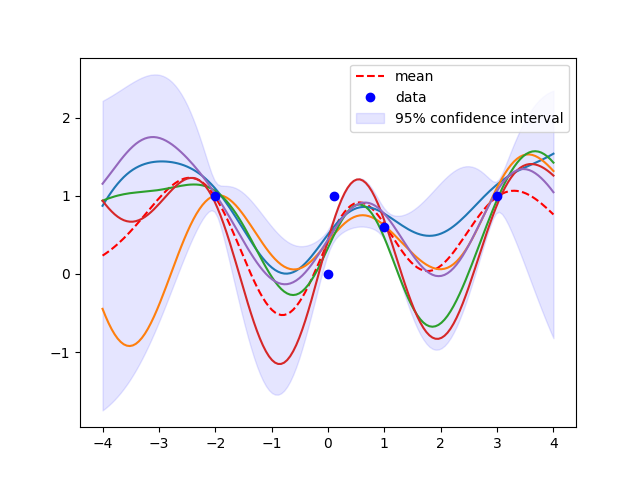
\includegraphics[width=.9\linewidth]{images/fig04.png}
\end{center}
\end{column}
\end{columns}
\end{frame}
\end{document}